\section{Reikningar}\label{ch::reikningar}

Við reikninga var miðað við eina plötu, þ.e. þegar aðskilnaður flata hefur átt sér stað. 

Byrjað var á ytri greiningu samsetningarinnar. Því ytra álag á hana er samhverft um miðju fæst að báður undir stöðukraftarnir eru $R_{A} = R_{B} = F/2$, sbr. mynd \ref{fig::forsendur}. Við útreikninga var miðað við að mesta spennur sem boltinn eða efnið þyldi væri flotmörk, þ.e. $n_y$ = 1. Mesta beygjuspenna sem hver plata þolir án þess að fara í flot er því í miðju samsetningarinnar. Út frá því má vinna mestan kraft sem hver plata þolir án þess að fara í flot.

\begin{equation}
	\sigma = \frac{M c}{I} = \frac{F l h}{4I} \Rightarrow F = \frac{4 \sigma I}{l h}
	\label{eq::1}
\end{equation}

Í jöfnu \ref{eq::1} er allt fastar nema flatartregðuvægið, I. Með því að lækka flatartregðuvægið mun mesti kraftur sem platan þolir fyrir flot minnka og því er ákveðið að bora ekki í miðja plötuna. Þessi kraftur, $F_{y,p}$, er því notaður sem lágmark þegar stærð, staðsetning og fjöldi bolta er valin. Flatartregðuvægið fyrir ferhyrnt þversnið $I = {1 \over 12}bh^3$.

\[
	F_{y,p} = \frac{4  \sigma_y I}{l h} = {\sigma_y b h^2 \over 3 l} = {210 MPa \cdot 5 mm \cdot \left(50mm\right)^2 \over 3 \cdot 200mm} = 4375N
\]

\subsection{Mismunandi tilvik semsetninga}

Þau tilvik sem þarf að skoða til viðbótar við þar sem samsetningin gefi sig eru þrenn

\begin{enumerate}
	\item Beygjuspenna á yfirborði þar sem borað verður
	\item Skerspenna sem boltar verða fyrir
	\item Leguspenna sem verkar á efnið í götunum
\end{enumerate}

Til að minnka beygjuspennu á yfirborði er ákveðið að hafa götin sem næst lóðréttum brúnum samsetningarinnar. Með því er vægisarmurinn frá undirstöðunum styttur, sem minnkar beygjuspennuna sbr. jöfnu \ref{eq::1}. Við þetta hækkar skerspennan í boltum og leguspennan í götum efnisins. Til að koma til móts við þessa spennuhækkun er ákveðið að hafa götin sem fjærst lágréttum brúnum samsetningarinnar, við það munu þær spennur lækkar, sbr. jöfnu \ref{eq::2}.

\begin{equation}
	F_n^{''} = {M r_n \over \displaystyle\sum_{i=1}^{k} r_i^2}
	\label{eq::2}
\end{equation}

Þar sem $F_n^{''}$ er skerkraftur sem verkar á bolta n sem er í fjarlægð $r_n$ frá flatarmiðju boltanna og k er fjöldi bolta í samsetningunni. Með þessu er hægt að finna leguspennu sem virkar á efnið og skerspennu sem virka á boltana. Reiknað voru þrjú tilvik af mismunandi samsetningu.

\begin{figure}
	\centering
	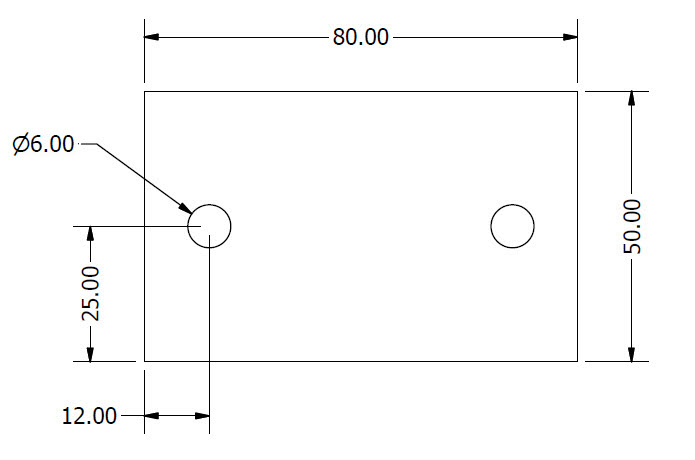
\includegraphics[width=0.5\textwidth]{2x6}
	\caption{Fyrsta reiknaða tilvik}
	\label{fig::2x6}
\end{figure}

\begin{figure}
	\centering
	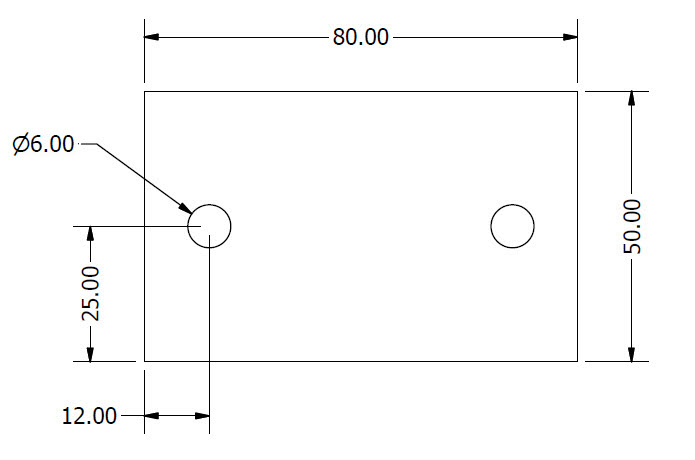
\includegraphics[width=0.5\textwidth]{2x6}
	\caption{Annað reiknaða tilvik}
	\label{fig::2x8}
\end{figure}

\begin{figure}
	\centering
	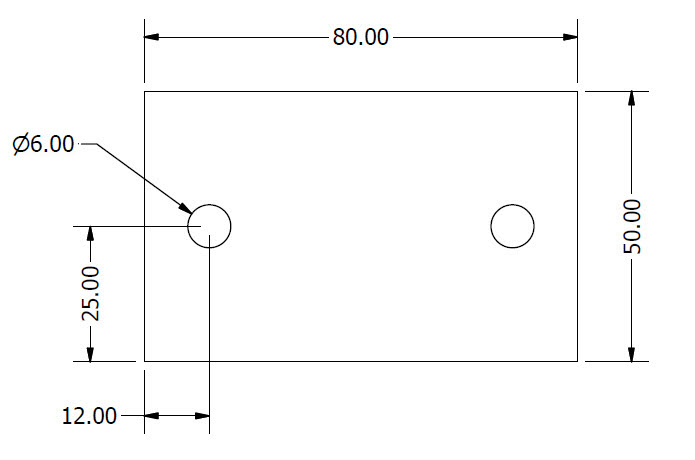
\includegraphics[width=0.5\textwidth]{2x6}
	\caption{Þriðja reiknaða tilvik}
	\label{fig::4x6}
\end{figure}